\documentclass[10pt,conference,compsocconf]{IEEEtran}

%\usepackage{times}
%\usepackage{balance}
\usepackage{amsmath,amssymb,graphicx,verbatim}
\usepackage{url}
\usepackage[norule]{footmisc}
\usepackage{adjustbox}
\usepackage{graphicx}% For figure environment

\usepackage{subcaption}
\usepackage{placeins}
\usepackage{float}
\setlength{\textfloatsep}{0.05cm}
\setlength{\intextsep}{8pt}
\begin{document}
\title{Can You Factor in your Neighbours? \\
\large A Hybrid Collaborative Filtering Algorithm}
\author{
  Fizza Zafar, Supraja Sridhara\\
  Department of Computer Science, ETH Zurich, Switzerland (Team Name: Duel)
}

\maketitle 

\begin{abstract}
Collaborative filtering is a technique used by recommendation systems, wherein ratings of other users and items are used to predict the rating for a given (user, item) pair. To this end, popular collaborative filtering algorithms use matrix factorization and neighbourhood based methods. We propose a novel approach that combines ideas of both factorization and neighbourhood based methods. We obtain ratings by considering hidden factors for the overall ratings matrix as well as sub-matrices obtained by clustering users and items. We evaluate our approach on the provided dataset and compare it to existing approaches. On the given data, this approach gives better performance than other existing algorithms. 
\end{abstract}

\section{Introduction}
Web based activity, such as e-commerce and online content distribution has increased drastically in the last decade resulting in a vast amount of content becoming available over the internet. This has made filtering relevant information a cumbersome task for users. To this end, recommendation systems are used by a variety of applications to serve personalized content to users. Effective recommendation systems exploit information about users' preferences to provide personalized content. Two techniques, content-based and collaborative filtering, are used by recommendation systems. Content based filtering depends on the users' specification of interests whereas collaborative filtering systems predict a user's preferences based on data from other users and/or items.

Due to their vast applicability, a large number of collaborative filtering  algorithms have been proposed in literature. These span correlation, clustering and matrix factorization based techniques, as well as their hybrids. The correlation and clustering based techniques use different metrics to identify similar users/ items and predict preferences based on them. Correlation based approaches are computationally expensive as they require pairwise correlation calculations whereas clustering based approaches are sensitive to initialization and do not take into account item synonymy. On the other hand, factorization based methods assume that there are unobserved factors that explain the rating given to different items by different users. They express both users and items in terms of these unknown factors. User ratings are predicted based on a low-rank approximation of the ratings matrix. We propose a novel method that predicts ratings based on global latent factors as well as those specific to a particular group of users/items. Our proposed algorithm gives a lower Root Mean Squared Error (RMSE), evaluated over the public test set on Kaggle.

In subsequent sections, we formulate the problem formally (section \ref{sec:problem}), outline existing approaches (section \ref{sec:existing_approaches})  and our proposed solution (section \ref{sec:proposed_method}). We evaluate all these techniques (section \ref{sec:results}) and, finally, discuss the results we obtained from them ( section \ref{sec:discussion}).

\section{Problem Formulation}\label{sec:problem}
Given a sparse matrix $A \in \mathbb{R} ^{m \times n}$ such that $A_{ij} \in [1,5] $ represents the rating of user $i$ for item $j$, we need to find a dense matrix  $B \in \mathbb{R} ^{m \times n}$ with $B_{ij} \in [1,5] $ such that it most closely approximates the true (unseen) dense ratings matrix. We consider $A$ to be a partially observed version of the true dense matrix $R$. The goal is to find $B$ such that it most closely approximates $R$

\section{Baseline Models}\label{sec:existing_approaches}
We evaluated a variety of models, described below. For most of these methods, we used implementations provided in the Python Surprise \cite{Surprise} library.
% Mean Imputation, NMF, SlopeOne, CoClustering, ALS (biases + mean), AutoRec, KNN, SVDpp, <some fancy name for our approach> 
\subsection{Random Value Imputation}
The simplest solution that we implemented randomly sampled from a normal distribution over the training data.
$$r_{ij} \sim N(\mu, \sigma^{2})$$ where $\mu$ is the average observed rating and $\sigma^{2}$ is its variance.

\subsection{Mean Value Imputation}
Next, we predicted missing rating as the sum of mean of all observed ratings and the user/ item bias.

    $$r_{ij} = \mu + b_{i} + b_{j}$$
The algorithm uses Alternating Least Squares (ALS)  to find optimal values for the user and item biases such that the (regularized) mean squared error over observed ratings is minimized.

\subsection{Matrix Factorization Methods}
Matrix factorization is one of the most prominent and effective techniques used for collaborative filtering. These models map users and items to the same latent factor space and unknown ratings are predicted as dot product of the concerned user and item embedding. They find $U \in \mathbb{R}^{m \times k}$, and $V \in \mathbb{R}^{n \times k}$ such that 

    $$A \approx UV^T$$

Different matrix factorization techniques find the best approximation of A under different constraints and objective functions. In order to avoid over-fitting, we regularized the factors. We now describe each of them.

\subsubsection{Singular Value Decomposition}
Singular Value Decomposition \cite{koren, RSH} of a matrix $A$ consists of three matrices U,D and V such that
    $$X = UDV^T$$
where $U \in \mathbb{R}^{m \times m}, D \in \mathbb{R}^{m \times n}$ and  $V \in \mathbb{R}^{n \times n}$. Matrices U and V are the user and item embeddings, respectively and D is the diagonal matrix of singular values of A. It represents the strength of each concept in explaining A. 

%TODO: Mention parameters (number of components, solver etc.)
\subsubsection{SVD with Implicit Feedback}
SVDpp \cite{RSH,SVDpp}, on top of the original SVD, this incorporates implicit feedback i.e. the fact that a user chose to rate a particular item, regardless of the rating value.

\subsubsection{Non-Negative Matrix Factorization}
Similar to other factorization techniques, NMF \cite{NMF} factorizes the ratings matrix into two lower rank matrices, minimizing the difference between the original and the low-rank approximation. However, it constrains the factor matrices to be non-negative as they are interpreted as probabilities. We used a (regularized) Stochastic Gradient Descent procedure to get the factor matrices. 

% \subsection{Slope One}
% Slope One \cite{SlopeOne} is a linear predictor that predicts ratings based on those of other items by user $i$ as other ratings of item $j$ by other users. It is a simple model based method that makes use of the average rating differential to predict ratings for a particular user and item. 

\subsection{K-Nearest Neighbors}
This approach predicts ratings for a particular user, item combination based on the ratings by other similar users (user-based), items (content-based) or a hybrid of both. The idea is that like-minded users will rate items on a similar scale and similar items are more likely to have similar ratings. Since there is no additional data about users/items, similarity is inferred from the available ratings.  $r_{ij}$ is predicted as the average rating of item j by 40 users most similar to user i. We used mean squared difference similarity metric for finding the nearest neighbour. 

\subsection{Neural Network Based Approaches}
Learning techniques are used in collaborative filtering, owing to their ability to learn non-linearity in the data. Deep neural networks are used to extract semantic information reflecting user-user, item-item and user-item correlation. We used the fastAI \cite{FastAI, FASTAIPaper} framework to train neural networks of different configurations, varying the number of layers, units per layer and activation functions. We also evaluated predictions by AutoRec, one of the state-of-the-art neural network frameworks for collaborative filtering. AutoRec \cite{AutoRec} is a collaborative filtering model based on the autoencoder paradigm. The algorithm uses back-propagation to account for ratings being only partially observed and  regularises the learned parameters to prevent overfitting. In contrast to matrix factorization approaches, the item-based AutoRec model embeds only items into latent spaces and can learn nonlinear latent representations through its activation function.

\section{Proposed Method}\label{sec:proposed_method}
Matrix factorization algorithms, while widely popular, try to find latent factors that accurately describe all users and items. Neighbourhood models, on the other hand, base ratings on user/item similarity, ignoring the underlying structure of the ratings matrix. Based on the ideas presented in \cite{MPMA}, we propose a hybrid method that predicts ratings based on 1) a user's ratings of all other items, 2) the strength of latent factors that describe all users/items and 3) the strength of latent factors that describe only a particular sub-group of users/items. The final rating blends all the above. The complete method is illustrated in Figure \ref{fig:overview}(a). We now describe the algorithm in detail. 


\begin{figure}[t]
  \centering
  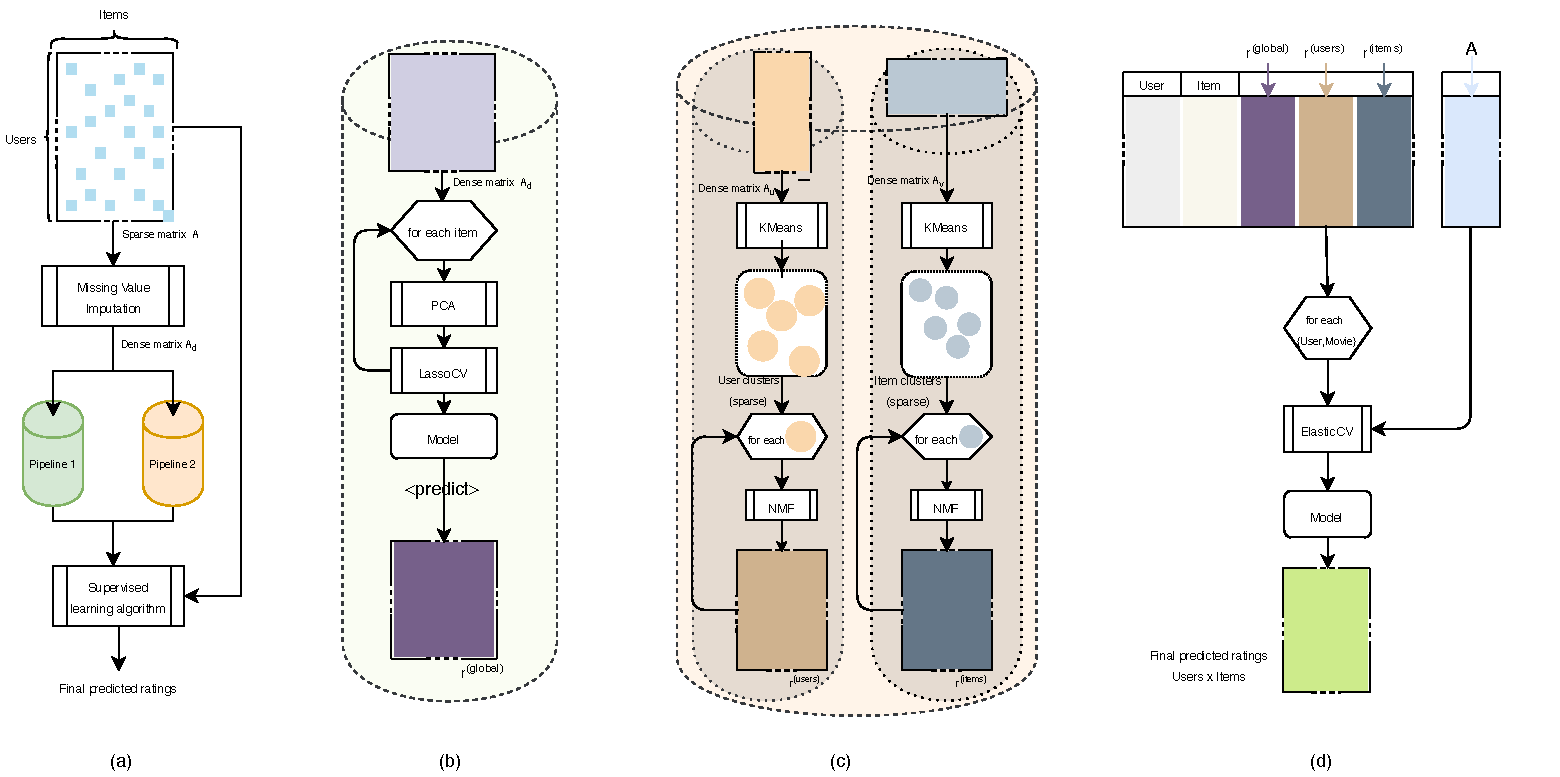
\includegraphics[height=6cm,width=0.5\textwidth]{cil_sample/figures/Algorithm.pdf}
  \caption{(a) The algorithm performs matrix factorization before branching into two independent pipelines. The pipelines then converge to solve a supervised learning problem. (b) Pipeline 1 performs PCA and LassoCV regression on the dense matrix to produce $r^{(global)}$ (c) Pipeline 2 has 2 sub-pipelines that perform clustering and matrix factorization to produce $r^{(user)}$ and $r^{(item)}$ (d) The final stage takes as input \{$r^{(global)}, r^{(user)}, r^{(item)}$\} and uses supervised learning methods to generate final predictions}
  \label{fig:overview}
\end{figure}

\textbf{Pipeline 1}:
This pipeline is illustrated in Figure\ref{fig:overview}(b). It can be divided into two phases: Imputation and Regression. We use NMF to impute unobserved values and transform the sparse matrix $A$ into a dense matrix $A_d$. $A$ and $A_d$ differ only in the unobserved values. In the regression phase, as described in \cite{RSH}, we independently fit regularized regressions on all columns of $A_d$, using all the other columns as predictor variables. Since the dataset has 1000 items, the feature matrix has a high dimensionality. In order to make the problem more tractable, we perform principal component analysis on it to reduce dimensionality while preserving the information from all columns. We use Lasso regularization in the linear models and select the regularization parameter using cross-validation. We call the output ratings matrix $r^{(global)}$

\textbf{Pipeline 2}:
Matrix factorization returns two factor matrices representative of user and item embedding independently. We use these as indicators of similarity between users/items. We cluster users and items based on the columns of the user and item embeddings, respectively, followed by factorization of the sparse sub-matrix obtained for each cluster. We define a sub-matrix for user cluster $u_1$ as all the entries in $A$ corresponding to users in $u_1$. A parallel definition holds for the items sub-matrix. We call the output ratings matrix based on user and item clusters $r^{(user)}$ and $r^{(item)}$ respectively. The 2 phases of this pipeline are illustrated in Fig\ref{fig:overview}(c).


\textbf{Combining both pipelines}: We then combine the three predictions for every user-item pair. The final rating is given as:
$$ r_{ij} =  \pi_{0}r_{ij}^{(global)} + \pi_{1}r_{ij}^{(user)} + \pi_{2}r_{ij}^{(item)}$$
We find the optimal parameters $\pi$ that minimize the sum of squared errors over the observed ratings.  With the observed ratings in the sparse matrix $A$ as the dependent variable and the predictions \{$r_{ij}^{(global)},r_{ij}^{(user)},r_{ij}^{(item)}$\} as independent variables the algorithm performs a regularized regression to determine the mixing weights for each of the three sub-components (see Fig\ref{fig:overview}(d)). 



\begin{figure}[h]
  \centering
  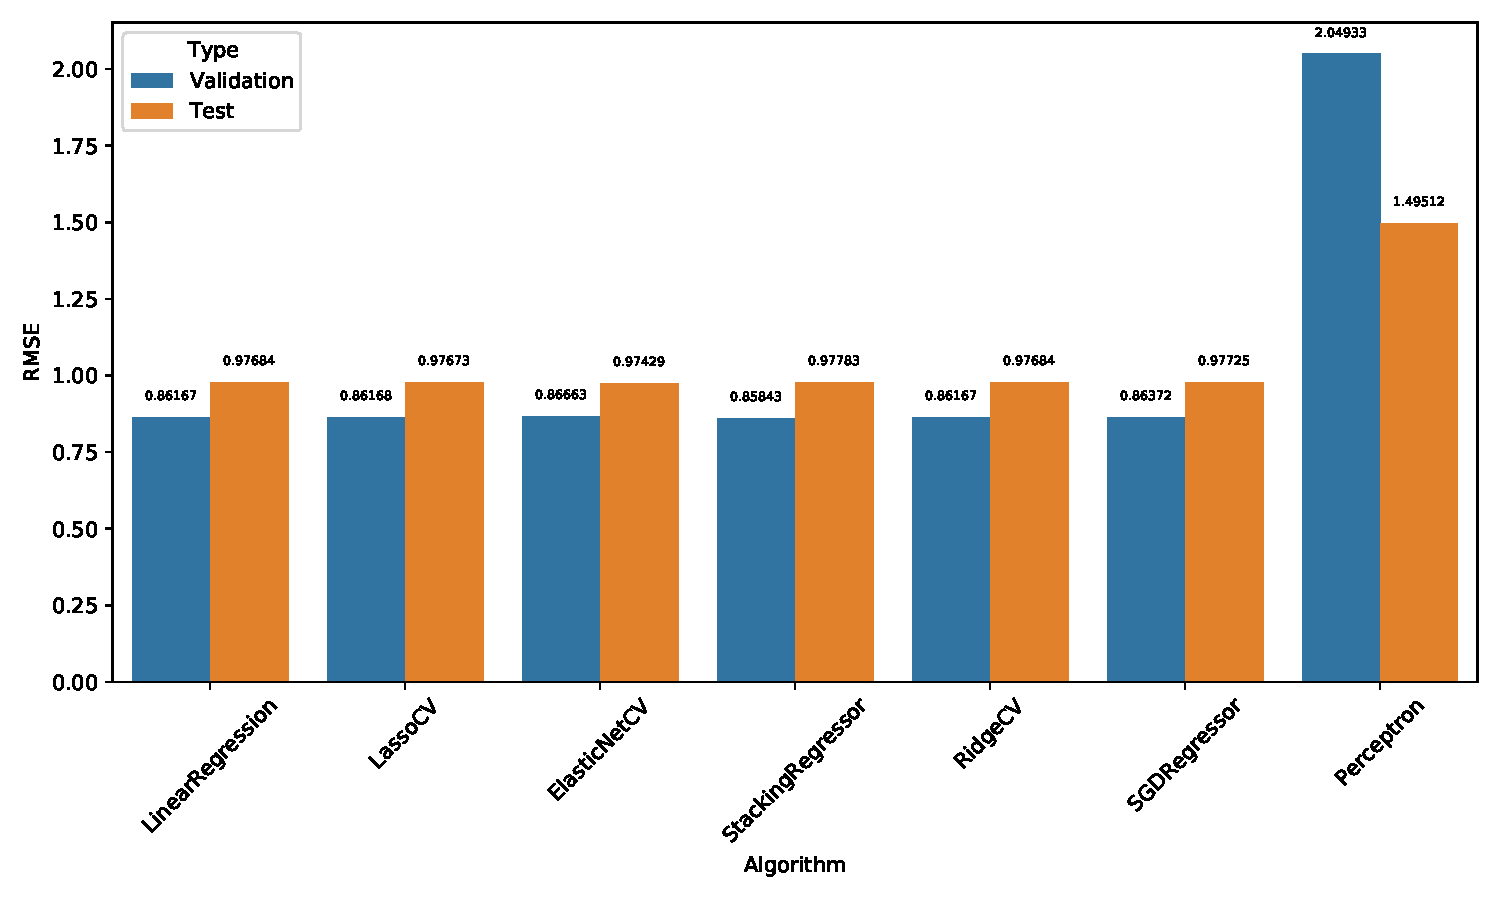
\includegraphics[height=3.5cm,width=0.5\textwidth]{cil_sample/figures/Models.pdf}
  \caption{RMSE scores for different blending models}
  \label{fig:models}
\end{figure}

\begin{figure}[h]
  \centering
  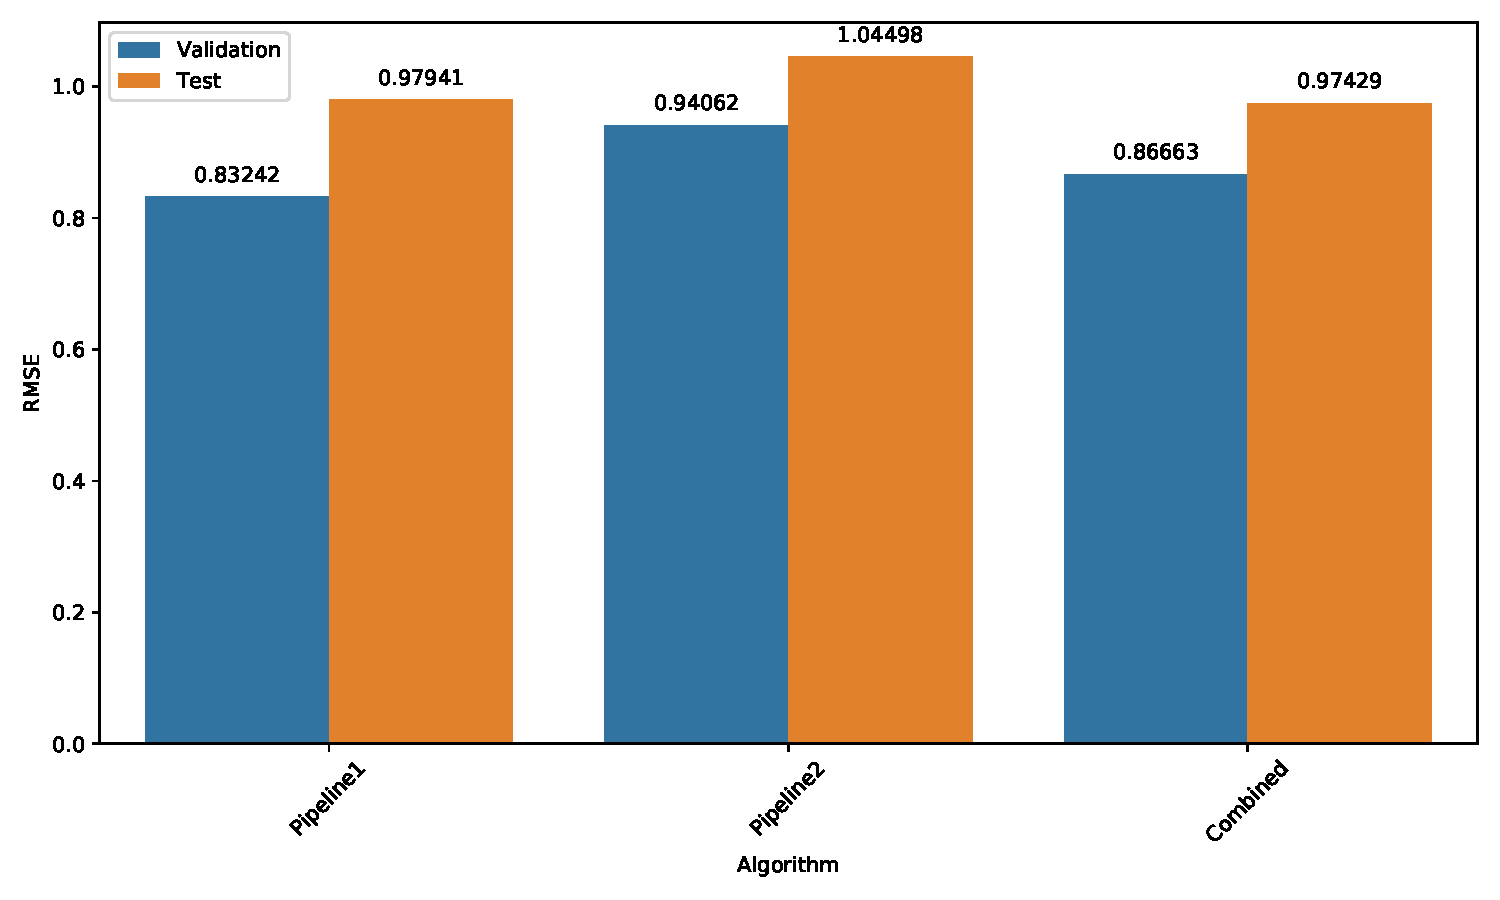
\includegraphics[height=3cm,width=0.4\textwidth]{cil_sample/figures/Pipelines.pdf}
  \caption{RMSE scores for evaluating pipelines separately}
  \label{fig:pipelines-separate}
\end{figure}


\section{Results}\label{sec:results}

\subsection{Parameter Tuning}
Due to constrained computational resources, we parameter tuned alternatively, first tuning the cluster-based parts of our algorithm (keeping the results of the first pipeline fixed) and then tuning NMF imputation on top of that (keeping the results of the previous pipeline fixed). Table \ref{table:params} summarizes the values of the different parameters we used to train our final model.

\begin{table}[H]
\centering
\begin{tabular}{|l|l||l|l|}
\hline
\textbf{Parameter Name} & \textbf{Value} & \textbf{Parameter Name} & \textbf{Value} \\ \hline
Global NMF epochs       & 185            & User NMF factors        & 30             \\ \hline
Global NMF factors      & 900            & Item clusters           & 2              \\ \hline
User clusters           & 7              & Item NMF epochs         & 10             \\ \hline
User NMF epochs         & 8              & Item NMF factors        & 30             \\ \hline
\end{tabular}\caption{Parameters to train final model} \label{table:params}
\end{table}



\textbf{Clustering and Sub-Matrix Factorization}: Figure \ref{fig:gridsearchlocal} shows the results for a grid search over number of clusters, factors and epochs used in Pipeline 2 (see Figure \ref{fig:overview}(c)). The grid search allowed us to narrow down possible parameter combinations which we then evaluated over the public test set to get the final combination. RMSE of different combinations on the public test set can be seen in Figure \ref{fig:localtest}. We chose the combination, given in Table \ref{table:params}, that gave the minimum test RMSE, .

\begin{figure}[H]
  \centering
  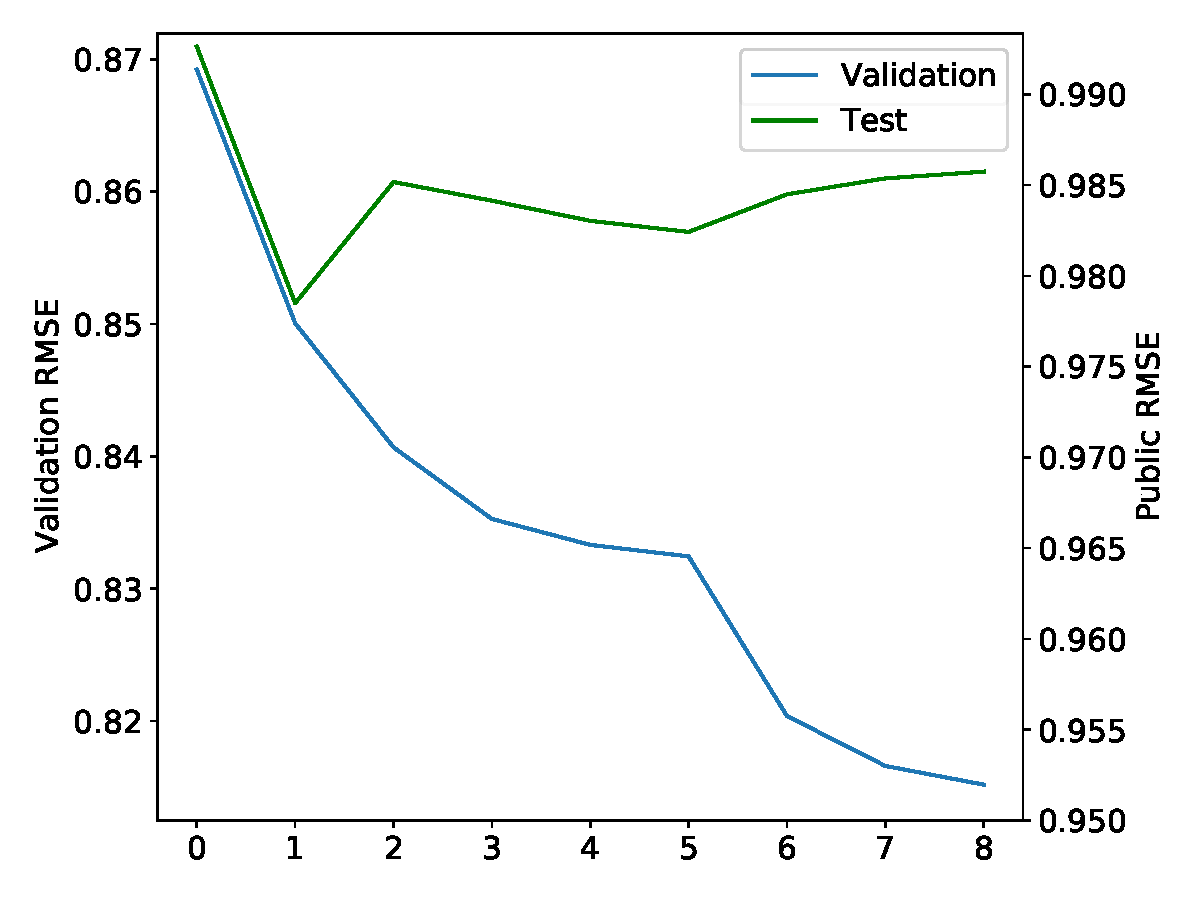
\includegraphics[scale=0.28]{cil_sample/figures/Local_params_valid_test.pdf}
  \caption{Validation and Test RMSE for different parameters of local factorization}
  \label{fig:localtest}
\end{figure}

\textbf{Imputation and Regression}: On top of the chosen parameters for the cluster-based part of the algorithm, we tried different parameters for NMF imputation. We performed a random search over the number of factors and the number of epochs for this NMF. In the first phase we searched the complete grid with factors $\in$ [100, 300] and epochs $\in$ [100, 300]. As expected, the performance of the algorithm improved with the number of factors. Moreover, for any given number of factors, epochs between 150 and 200 gave the best validation RMSE. In the second phase, we tried multiple combinations with factors $\in$ [700, 900] and epochs $\in$ [150,200]. The results of the 2 phases are summarized in Figure \ref{fig:gridsearchglobal}. Based on these findings, we evaluated the test RMSE for factors = 900 and epochs = [150,175,185,200] and found 900 factors and 185 to give the best performance. Table \ref{table:testrmse-global-epochs} gives the obtained Test RMSE for different epochs.
% Therefore, we fixed epochs and kept on increasing factors. As shown in Table \ref{table:testrmse-global}, RMSE improved with factors but we eventually observe diminishing returns to increasing factors. As a result, we chose 900 factors. In the next step, we fixed the factors at 900 and increased the epochs from 150 to 200. As seen in Table \ref{table:testrmse-global-epochs} we found that the RMSE is lowest at 185 epochs before it begins to increase again.


\begin{figure}[H]
  \centering
  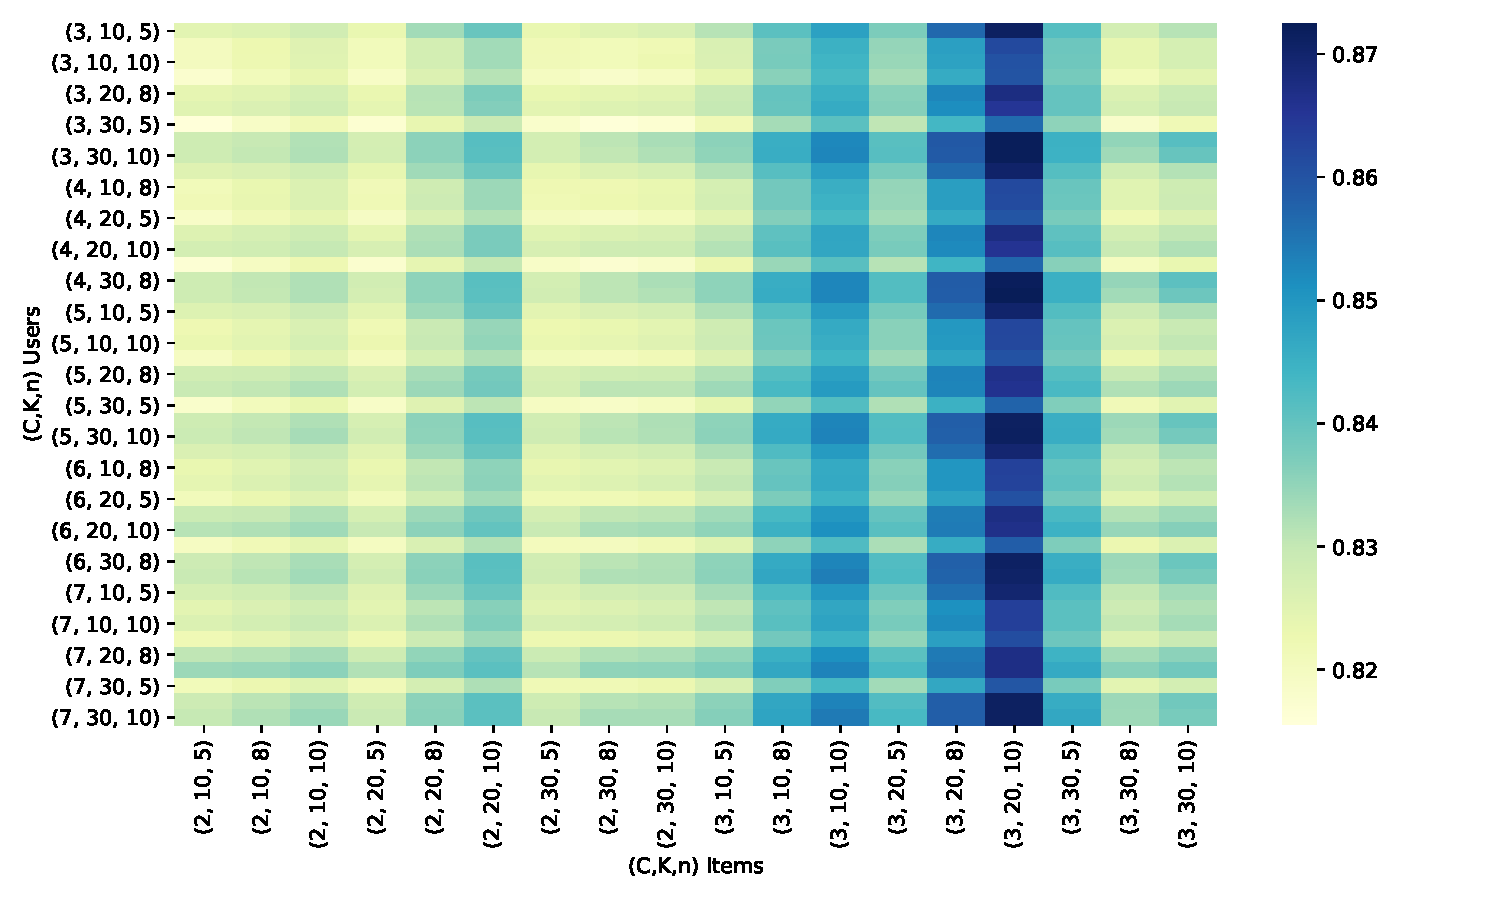
\includegraphics[height=4cm,width=0.5\textwidth]{cil_sample/figures/Local_params.pdf}
  \caption{RMSE scores for Number of Clusters, Hidden Factors, Number of Epochs (C,K,n) for user and item clusters, produced by grid search with 2 fold cross-validation}
  \label{fig:gridsearchlocal}
\end{figure}

\textbf{Blending Models}: We also evaluated the performance of different blending models that were available in Python's sklearn library \cite{sklearn}. The results are summarized in Figure \ref{fig:models}. We observe that non-linear methods overfit very easily whereas linear models generalize better. The best performance was given by ElasticNetCV which uses a combination of lasso and ridge regression, with the optimal regularisation parameter being found using cross-validation.


% \begin{figure}[h]
%   \centering
%   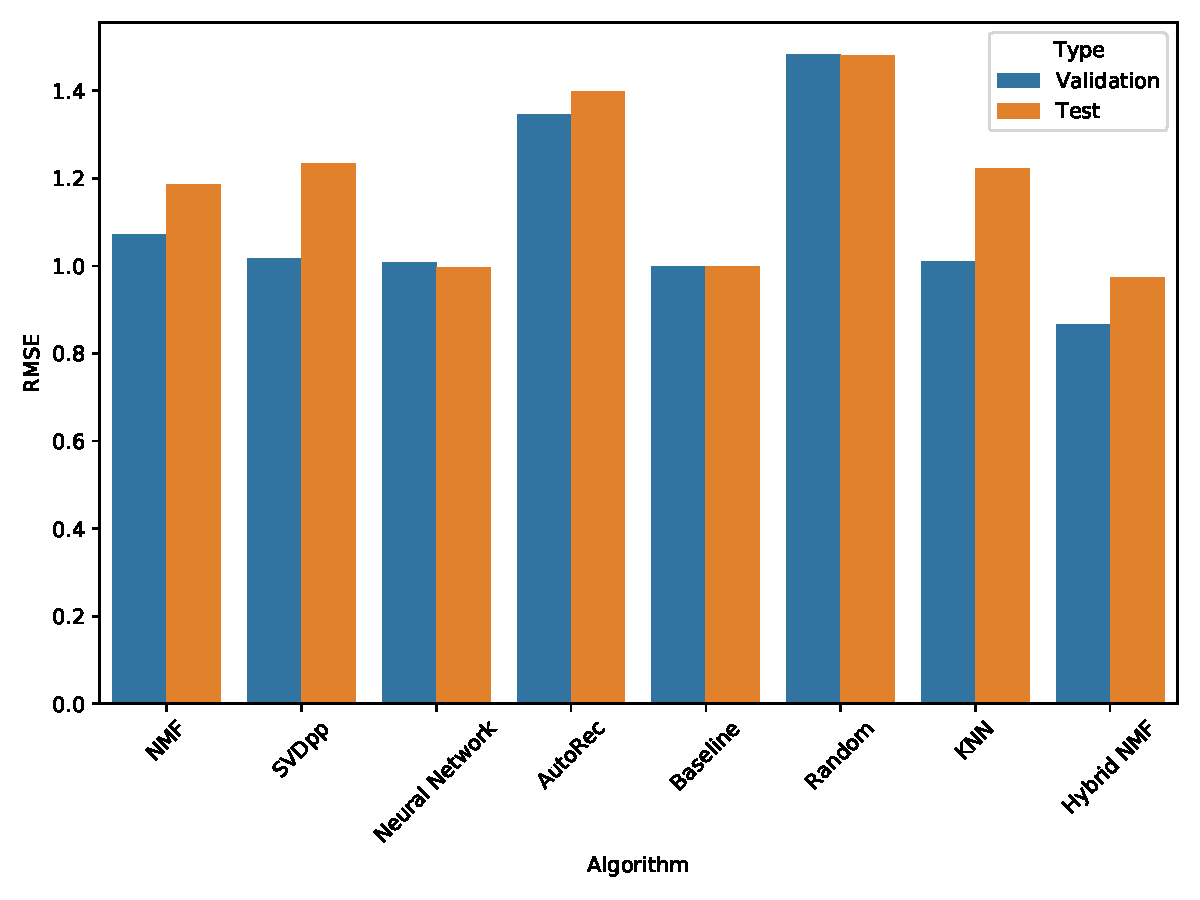
\includegraphics[scale=0.33]{cil_sample/figures/Baselines.pdf}
%   \caption{Comparison of different CF Algorithms}
%   \label{fig:baselines}
% \end{figure}

% \begin{table}[]
% \centering
% \begin{tabular}{|l|l|l|}
% \hline
%           & \textbf{Validation} & \textbf{Test} \\ \hline
% Pipeline 1 & 0.83242             & 0.97941       \\ \hline
% Pipeline 2 & 0.94062             & 1.04498       \\ \hline
% Combined   & 0.86663             & 0.97429       \\ \hline
% \end{tabular} \caption{Evaluating both pipelines separately} \label{table:pipelines-separate}
% \end{table}


\subsection{Evaluating the Effect of Blending}
To evaluate whether blending the local and global pipelines actually lead to an improvement in RMSE, we evaluated both separately on the test data set. In order to draw a fair comparison, we used the parameters that gave best results for each pipeline separately. Figure \ref{fig:pipelines-separate} gives an overview of the results. Combining both pipelines gives a better test RMSE than generating predictions from either pipeline independently. This implies that the model does indeed have something to gain from the latent factors discovered through clustering and sub-matrix factorization.

\begin{table}[H]
\centering
\resizebox{0.5\textwidth}{0.065\textheight}{%
\begin{tabular}{|c|c|c|c|}
\hline
\textbf{Algorithm} & \textbf{Validation} & \textbf{Test} & \textbf{Parameters}         \\ \hline
NMF                & 1.0714975                & 1.18537            & epochs = 200, factors = 200 \\ \hline
SVDpp              & 1.0168                   & 1.23459            & epochs = 200, factors = 200 \\ \hline
Neural Network     & 1.007911                 & 0.99635            & layers={[}200,128,64,16{]}  \\ \hline
AutoRec            & 1.3462                   & 1.39741            & epochs=1, hidden neurons=100, batch size=100                          \\ \hline
Baseline           & 0.9996473                & 0.99768            & method=ALS, epochs = 10     \\ \hline
Random             & 1.48162                  & 1.48097            & method=ALS, epochs = 10     \\ \hline
KNN                & 1.00912                  & 1.22238            & K = 40                      \\ \hline
Hybrid NMF                & 0.86663                  & 0.97429            & See Table \ref{table:params}                      \\ \hline
\end{tabular}
}\caption{Validation and Test rmse for different cf techniques}\label{table:baselines}
\end{table}

\subsection{Comparison to Baselines}
We evaluated our fine-tuned proposed approach against existing techniques discussed in Section \ref{sec:existing_approaches}. Table \ref{table:baselines} summarizes the results. The worst performance is given by the random sampling baseline that does not take into consideration the underlying structure of the ratings matrix at all. Neural network based models over-fit to the data very easily. We tuned the number of epochs to get the best performing value but were unable to further tune both approaches due to time and compute constraints. Individually, both neighbourhood and factorization based approaches do not perform very well. On the other hand, our hybrid model gives approximately 20\% improvement in RMSE compared to performance of either model in isolation.



\begin{figure}[h]
  \centering
  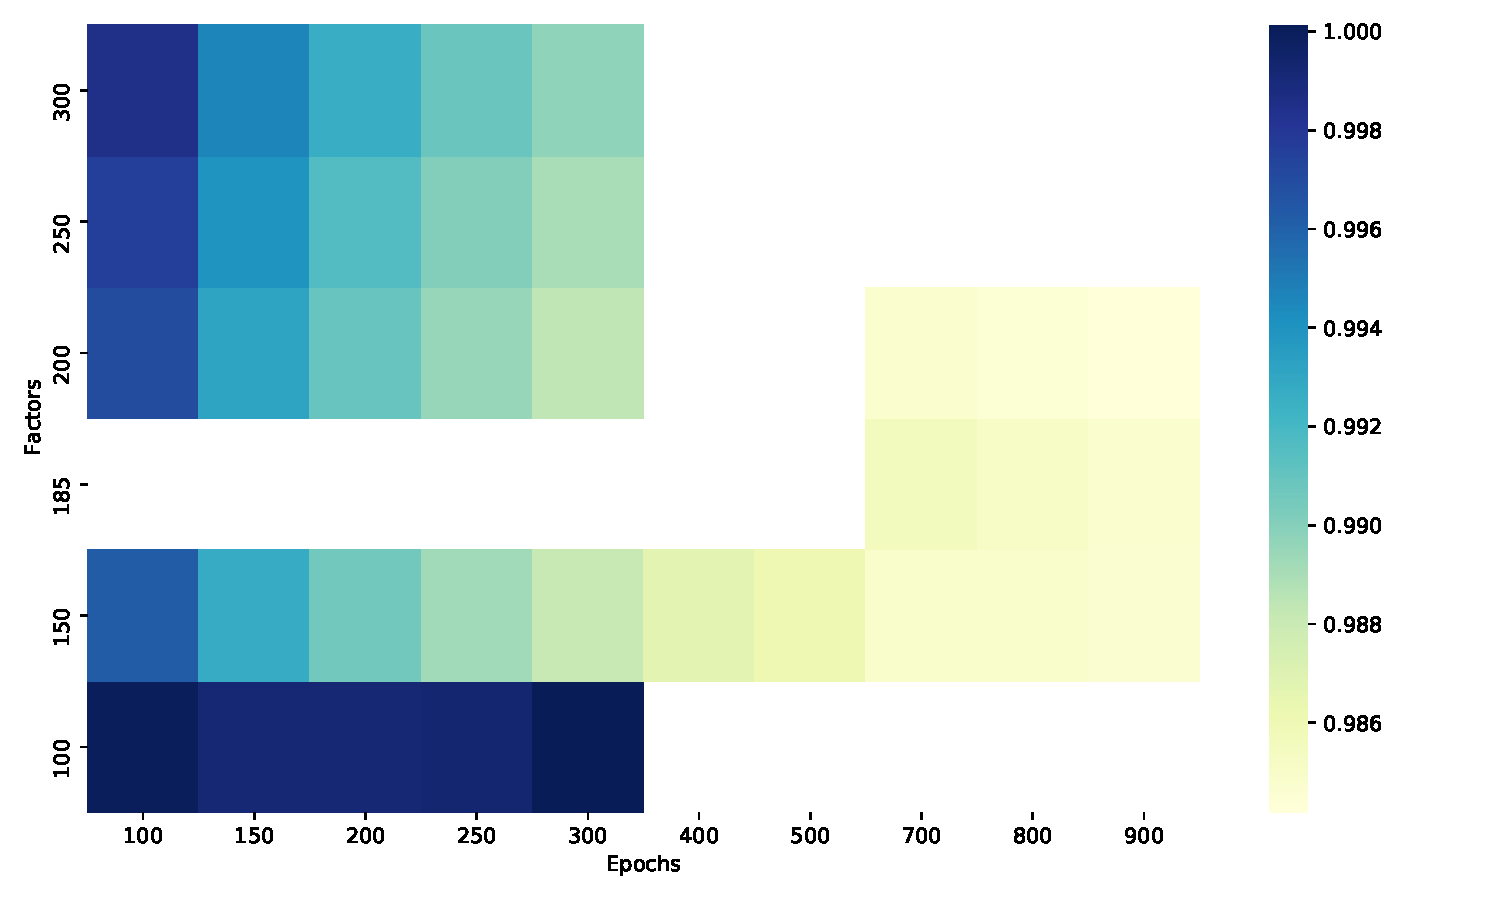
\includegraphics[height=3cm]{cil_sample/figures/Global_params.pdf}
  \caption{RMSE scores for epochs vs. factors of global NMF produced by grid search with 5 fold cross-validation}
  \label{fig:gridsearchglobal}
\end{figure}

% \begin{table}[]
% \centering
% \begin{tabular}{|l|l|}
% \hline
% Factors & Test RMSE \\ \hline
% 400     & 0.97716   \\ \hline
% 600     & 0.97663   \\ \hline
% 700     & 0.97644   \\ \hline
% 800     & 0.97643   \\ \hline
% 900     & 0.97639   \\ \hline
% \end{tabular}\caption{Test rmse for varying number of factors of global nmf}\label{table:testrmse-global}
% \end{table}

\begin{table}[h]
\centering
\begin{tabular}{|l|l|}
\hline
Epochs & Test RMSE \\ \hline
150     & 0.97639   \\ \hline
175     & 0.97472   \\ \hline
185     & 0.97429   \\ \hline
200     & 0.97449   \\ \hline
\end{tabular}\caption{Test rmse for varying number of epochs of global nmf for 900 factors}\label{table:testrmse-global-epochs}
\end{table}


% \begin{table}[]
% \centering
% \begin{tabular}{|l|l|l|}
% \hline
% \textbf{Model}    & \textbf{Validation} & \textbf{Test} \\ \hline
% LinearRegression  & 0.86167             & 0.97684       \\ \hline
% LassoCV           & 0.86168             & 0.97673       \\ \hline
% ElasticNetCV      & 0.86663             & 0.97429       \\ \hline
% StackingRegressor & 0.85843             & 0.97783       \\ \hline
% RidgeCV           & 0.86167             & 0.97684       \\ \hline
% SGDRegressor      & 0.86372             & 0.97725       \\ \hline
% Perceptron        & 2.04933             & 1.49512       \\ \hline
% \end{tabular}\caption{\label{table:models} Validation and Test RMSE for different blending methods} 
% \end{table}



 

%  Lastly, we tried different models for combining the local and global predictions that we got. We tried linear as well as non-linear models e.g. stacking regressor, neural network etc. However, we found that linear models performed the best. For linear regression, we tried different regularization techniques and parameters and found Elastic Net to be best performing. This model uses a combination of lasso and ridge regression giving equal weightage to both. The regularization parameter was chosen through cross-validation.

% -> Naive Results (w/o parameter tuning)
% -> Grid search + [heatmap] (9305 combinations) [point plt RMSE vs params]
% -> Tuning the imputation NMF [point plt RMSE vs params]
% -> Different Models (Simple Linear, Lasso, ElasticCV, Stacking Regressor, Perceptron) [bar chart with test and val rmse]
% -> Compare with baselines [bar chart with test and val rmse]
%

\section{Discussion}\label{sec:discussion}
% Strengths: - Comparable (Better) accuracy while reasonable training time. - Takes into account latent factors at the local level as well as broader hidden variables.
% Weaknesses: -
Our proposed method achieves better accuracy than existing models and is efficiently parallelizable as the different pipelines are independent. As a result, we do not expect the training time to become a performance bottleneck. The approach considers latent factors at both global and local levels. Since this encompasses a broad set of hidden variables we expect it to generalize well to unseen data.
We note that the usefulness of this method hinges on the assumption that the set of local factors has something to add to the set of global factors, in explaining the rating for a given (user, item) pair. In fact, we expect it to work best when these two sets are disjoint. In the event that one is a subset of the other, one of the pipelines may possibly become obsolete. 

\section{Summary} 
In this work we have presented a novel ensemble based approach to collaborative filtering that uses non-negative matrix factorization, clustering and regression. We combine these methods to capture both global and local latent factors. By comparing our solution to several existing approaches we have shown that it performs significantly better on the given dataset. We tried different blending methods and found cross-validated, elastic net regularized regression to give the lowest test RMSE. Further work can include investigating other matrix factorization and clustering approaches e.g. soft clustering to encompass a wider range of factors.

\bibliographystyle{IEEEtran}
\bibliography{paper}

\end{document}